
\section{SysML approach with Papyrus}

\subsection{Introduction to SysML with Papyrus}

\begin{comment}
short introduction to sysML language with references to  OMg specification and major document which describe it + short description of main concepts of SysML +  short description of particularities of SysML on papyrus. (parts of 07.1.3\_O7.1.7 may be reused). 
\end{comment}

\subsection{SysML in the project}

The proposal is to use SysML for the highest level of modelling:
\begin{description}
\item[Conception and design] Aim of the SysML model is to manage the gap  between prose system analysis and formal model dedicated to the design of on board unit. Thus the SysML model will provide a high level model associated to the system analysis, the SSRS and the API:
\begin{itemize}
\item Structure of the system, with physical and functional architecture will be described with \textit{Block Definition Diagrams} and \textit{Package Diagrams}
\item Logical interfaces between subsystems and between functions will be described with \textit{Internal Block Diagrams}
\item Data definition will be defined with \textit{Block Definition Diagrams}
\item Requirements will be defined and allocated with \textit{Requirements Diagrams}
\item High level Behaviour description will be described with \textit{State Machine Diagrams}
\end{itemize}
\item[Safety analysis] SysML model will provide an organic and a functional architecture of the system
\begin{itemize}
\item Functional Breakdown Structure will be defined with \textit{Block Definition Diagrams} and \textit{Internal Block Diagrams}
\end{itemize}
\item[Verification and Validation] SysML model will provide expected behavior of the system during execution: 
\begin{itemize}
\item Test Cases and execution traces will be defined with \textit{Sequence Diagrams}
\end{itemize}
\end{description}

This list can be completed, after the results of benchmark  of secondary tools, either by defining use of some diagrams for other activities (for example for safety or VnV) or by defining methods and tools to use to complete SysML (for example for requirements management or database definition).

\subsection{Selection of used diagrams}

SysML diagrams that can be used for modeling are:
\begin{itemize}
\item \emph{Package Diagram}: Structure description
\item \emph{Block Definition Diagram} (BDD): Structure description
\item \emph{Internal Block Diagram} (IBD): Structure description
\item \emph{Sequence Diagram}: Test case, execution trace, counter
  example, etc.
\item \emph{State Machine Diagram}: Behaviour description
\item \emph{Requirement Diagram}: Requirements description
\end{itemize}

The following other SysML diagrams \emph{cannot} be used:
\begin{itemize}
\item \emph{Parametric Diagram}
\item \emph{Activity Diagram}
\item \emph{Use Case Diagram}
\end{itemize}

\subsubsection{Remarks for all diagrams}

Following elements are allowed on all kinds of diagrams:
\begin{itemize}
\item Comment Note
\end{itemize}

\subsubsection{Notes on selected diagrams}

The diagrams and diagram elements of SysML have been chosen because
(1) they are supported by Papyrus v0.10.0 used in Eclipse Kepler
release and because (2) they are the minimal subset of SysML needed
for a proper system description and V\&V activities.

In the future, we can decide to augment the chosen SysML subset
because Papyrus offers new capabilities and because new elements are
needed. This can been done at project level following a procedure
which is not yet decided.

\subsection{Restrictions on Package Diagram}

Note: The naming of the nodes and paths of this section and the
following one is the same as Annex A of book ``A Practical Guide to
SysML''.


\begin{figure}[ht]
  \centering
  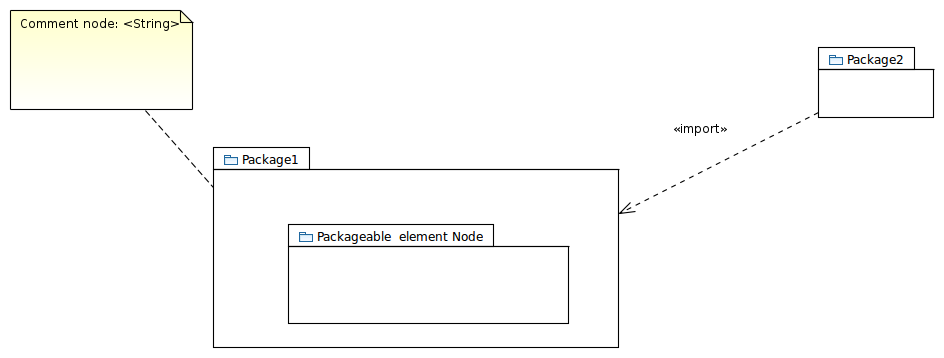
\includegraphics[width=\textwidth]{images/PackageDiagram.PNG}
  \caption{Package Diagram}
  \label{fig:package diagram}
\end{figure}


The following Package Diagram nodes and paths can be used for
modelling:
\begin{itemize}
\item Comment Note \sysmlicon{Comment.png}
\item Package Node \sysmlicon{Package.png}
\item Packageable Element Node
\item Import Path \sysmlicon{PackageImport.png}
\end{itemize}

The following items \emph{cannot} be used:
\begin{itemize}
\item Model Node
\item View Node
\item Viewpoint Node
\item Containenement Path
\item Dependency Path
\item Conform Path
\item Metamodel Node
\item Metaclass Node
\item Model Library Node
\item Stereotype Node
\item Profile Node
\item Generalization Path
\item Extension Path
\item Associatin Path
\item Reference Path
\item Profile Application Path
\end{itemize}

\subsection{Restrictions on Block Definition Diagram}



\begin{figure}[ht]
  \centering
  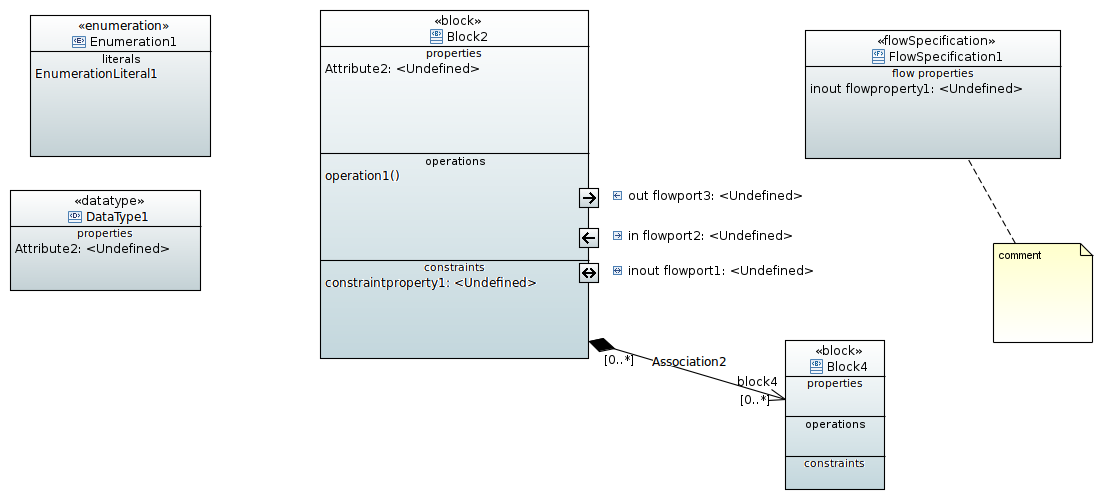
\includegraphics[width=\textwidth]{images/BDDDiagram.PNG}
  \caption{Block Description Diagram}
  \label{fig:Bdd}
\end{figure}



The following Block Definition Diagram nodes and paths can be used for
modelling:
\begin{itemize}
\item Block Node \sysmlicon{Block.png}
\item Enumeration Node \sysmlicon{Enumeration.png}
\item Block Node with ``datatype'' Stereotype \sysmlicon{DataType.png}
\item Composite Association Path \sysmlicon{Association_composite.png}
\item Flow Specification Node \sysmlicon{FlowSpecification.png}
\item Atomic Flow Port Node \sysmlicon{FlowPort.png}  \sysmlicon{FlowPort_INOUT.png} \sysmlicon{FlowPort_IN.png} \sysmlicon{FlowPort_OUT.png}
\end{itemize}

The following items \emph{cannot} be used:
\begin{itemize}
\item Quantity Kind and Unit Nodes
\item Value Type Node
\item Actor Node
\item Interface Block Node (SysML 1.3)
\item Interface Node
\item Signal Node
\item Interface Compartments for Block Node
\item Reference Association Path
\item Association Block Path and Node
\item Generalization Path
\item Full Port Node
\item Proxy Port Node
\item Proxy Port Node With Interfaces
\item Port Compartments for Block Node
\item Nonatomic Flow Port Node
\item Block Node with Constraint Compartment
\item Constraint Block Node
\item Activity Node
\item Activity Composition Path
\item Object Node Composition Path
\item Instance Specification Node
\item Association Instance Specification (Link) Path
\end{itemize}

\subsection{Restrictions on Internal Block Diagram}



\begin{figure}[ht]
  \centering
  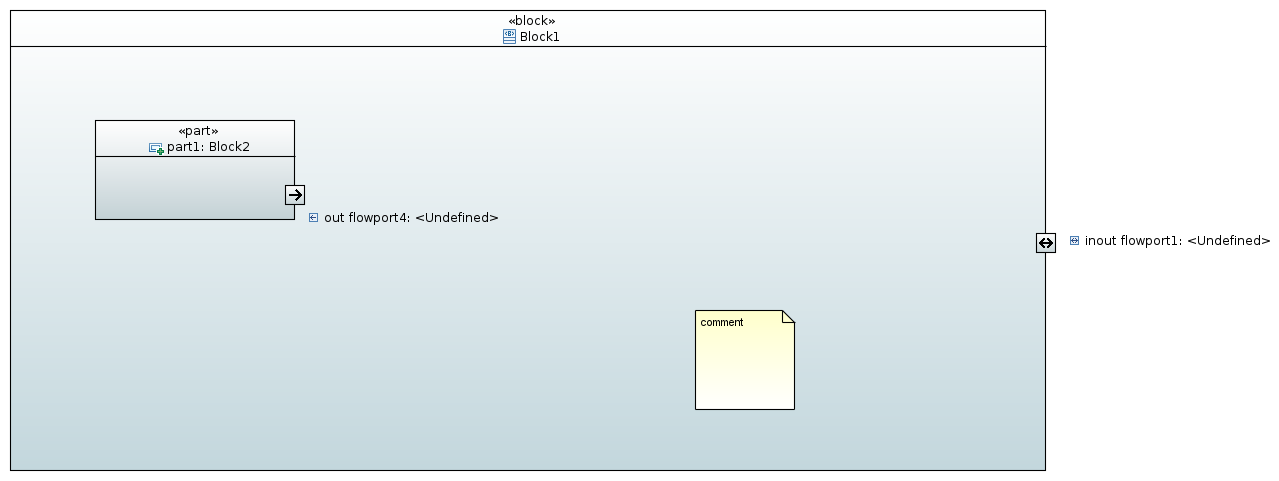
\includegraphics[width=\textwidth]{images/IBDDiagram.PNG}
  \caption{Internal Block Diagram}
  \label{fig:ibd}
\end{figure}


The following Internal Block Diagram nodes and paths can be used for
modelling:
\begin{itemize}
\item Part Node \sysmlicon{Property.png}~\textsf{Part}
\item Connector Path
\end{itemize}

The following items \emph{cannot} be used:
\begin{itemize}
\item Actor Part Node
\item Reference Node
\item Participant Property Node
\item Value Property Node
\item Connector Property Path and Node
\item Item Flow Node
\end{itemize}

\subsection{Restrictions on Sequence Diagram}



\begin{figure}[ht]
  \centering
  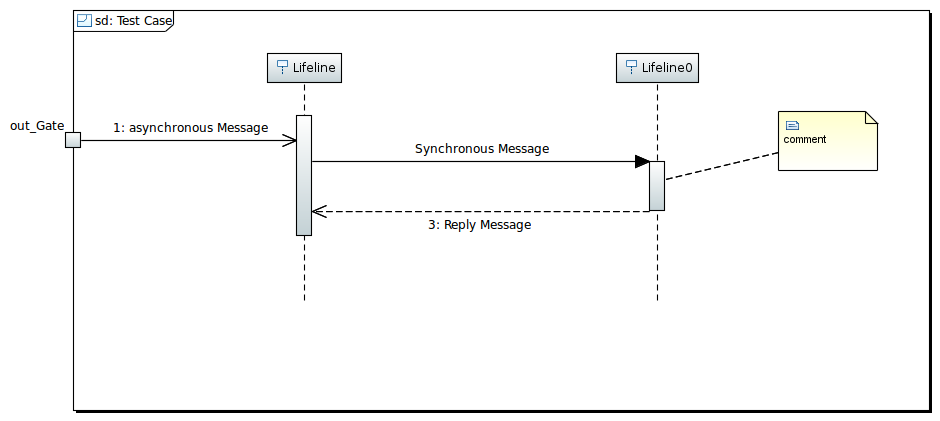
\includegraphics[width=\textwidth]{images/SequenceDiagram.PNG}
  \caption{Sequence Diagram}
  \label{fig:sd}
\end{figure}


The following Sequence Diagram nodes and paths can be used for
modelling:
\begin{itemize}
\item Lifeline Node
\item Synchronous Message
\item Asynchronous Message
\item Reply Message
\end{itemize}

The following items \emph{cannot} be used:
\begin{itemize}
\item Single-compartment Fragment Node
\item Multi-compartment Fragment Node
\item Filtering Fragment Node
\item State Invariant Symbol
\item Interaction Use Node
\item Lost Message Path
\item Found Message Path
\item Activation Node
\item Create Message Path
\item Destroy Event Node
\item Coregion Symbol
\item Duration Observation Symbol
\item Duration Constraint Symbol
\item Time Observation Symbol
\item Time Constraint Symbol
\end{itemize}

\subsection{Restrictions on State Machine Diagram}



\begin{figure}[ht]
  \centering
  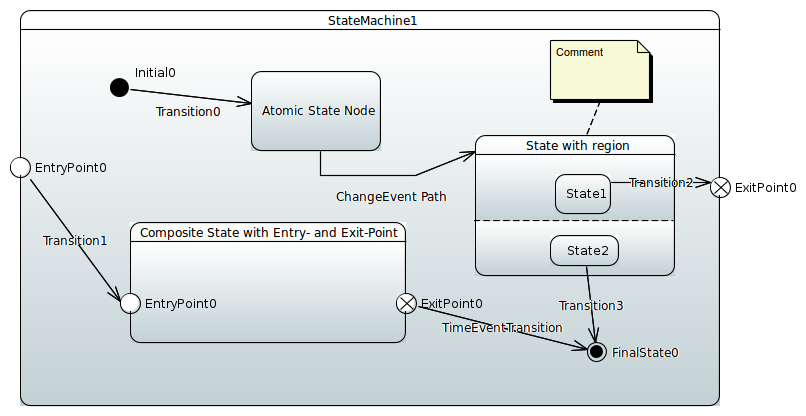
\includegraphics[width=\textwidth]{images/StateMachineDiagram.PNG}
  \caption{State Machine Diagram}
  \label{fig:sm diagram}
\end{figure}


The following State Machine Diagram nodes and paths can be used for
modelling:
\begin{itemize}
\item State Machine with Entry- and Exit-Point Pseudostate Nodes
\item Atomic State Node
\item Composite State with Entry- and Exit-Point Pseudostate Nodes
\item Composite State Node with Multiple Region
\item Initial Pseudostate Node
\item Final State Node
\item Time Event Transition Path
\item Change Event Transition Path
\item Constraint Node (for transition guard)
\end{itemize}

The following items \emph{cannot} be used:
\begin{itemize}
\item Sub-State Machine Node with Connection Points
\item Terminate Pseudostate Node
\item Choice Pseudostate Node
\item Junction Pseudostate Node
\item Trigger Node
\item Action Node
\item Send Signal Node
\item Join Pseudostate Node
\item Frok Pseudostate Node
\item History Pseudostate Node
\item Signal Event Transition Path
\item Call Event Transition Path
\end{itemize}

\subsection{Restrictions on Requirement Diagram}

\begin{figure}[ht]
  \centering
  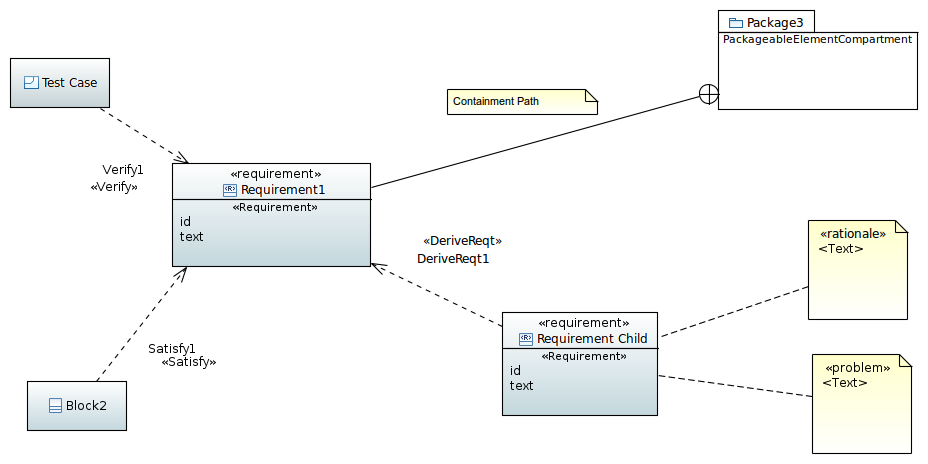
\includegraphics[width=\textwidth]{images/RequirementDiagram.PNG}
  \caption{Requirement Diagram}
  \label{fig:req diagram}
\end{figure}


The following Requirement Diagram nodes and paths can be used for
modelling:
\begin{itemize}
\item Requirement Node
\item Package Node
\item Containment Path
\item Derivation Path
\item Satisfaction Path
\item Verification Path
\item Rationale Callout
\item Problem Callout
\end{itemize}

The following items \emph{cannot} be used:
\begin{itemize}
\item Requirement Related-Type Node
\item Trace Compartment
\item Test Case Node
\item Refinement Path
\item Trace Path
\item Copy Path
\item Trace Callout
\item Derivation Callout
\item Verification Callout
\item Statisfaction Callout
\item Refinement Callout
\item Master Requirement Callout
\end{itemize}



\subsection{Model patterns}

For \emph{Modelling} activity, the modeler shall only use:
\begin{itemize}
\item \emph{Package Diagram}
\item \emph{Block Definition Diagram} (BDD)
\item \emph{Internal Block Diagram} (IBD)
\item \emph{State Machine Diagram}
\item \emph{Requirement Diagram}
\end{itemize}

For \emph{V\&V} activities, one shall only use:
\begin{itemize}
\item \emph{Package Diagram}
\item \emph{Block Definition Diagram} (BDD)
\item \emph{Internal Block Diagram} (IBD)
\item \emph{Sequence Diagram}
\item \emph{Requirement Diagram}
\end{itemize}


\begin{comment}
FIXME: Example of patterns to use.

\end{comment}


% LocalWords:  SysML
